
\begin{figure}[h] %  figure placement: here, top, bottom, or page
   \centering
   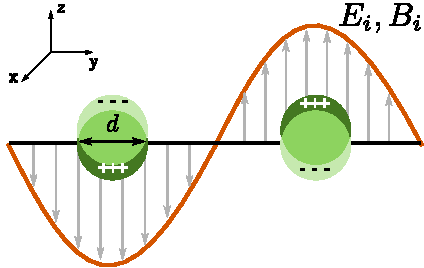
\includegraphics[width=0.49\textwidth]{lspr.pdf} 
   \caption{Localized Surface Plasmon Resonance (LSPR) scheme. LSPR is an 
            optical phenomenon that ocurrs when light shines on conductive 
            nanoparticles that are smaller than the wavelength of the incident 
            light. The free electrons on the surface of the nanoparticle are 
            excited by the incoming electric field oscillating with it and 
            creating plasmons \textcolor{blue}{this figure is from another paper. We should redo it or cite.}.}
   \label{fig:lspr}
\end{figure}




